\documentclass{article}
\usepackage[english]{babel}
\usepackage{csquotes}

%%% Functional packages
\usepackage{amsmath, amssymb, amsthm, mathtools}
\usepackage{physics, siunitx}
\usepackage{graphicx}
    \graphicspath{{plots/}}
\usepackage[subfolder]{gnuplottex}
\usepackage[font=small]{caption}
\usepackage{subcaption}
\usepackage{overpic}
\usepackage{tikz}
    \usetikzlibrary{arrows, intersections, calc}


%%% Configuration packages
%\usepackage{fullpage}
\usepackage[export]{adjustbox}      % For centering wide figures

\usepackage[
    pdfusetitle,
    colorlinks
]{hyperref}

\usepackage[
    backend=biber,
    style=numeric,
    giveninits=true,
    sorting=none,
    mincrossrefs=100, % do not add parent collections
]{biblatex}
\addbibresource{directional_solidification.bib}

\title{Stability analysis in directional solidification}
\author{Oleg Rogozin}

%%% Problem-specific aliases
\newcommand{\liq}{\text{L}}
\newcommand{\sol}{\text{S}}
\newcommand{\qL}{q_\liq}
\newcommand{\qS}{q_\sol}
\newcommand{\pL}{p_\liq}
\newcommand{\pS}{p_\sol}
\newcommand{\hV}[1][\qty(\bar{V})]{\vphantom{#1}\mathrlap{\smash{\hat{V}}}V}
\newcommand{\hG}[1][\qty(\bar{G})]{\vphantom{#1}\mathrlap{\smash{\hat{G}}}G}

%%% Bold symbols
\newcommand{\bn}{\vu*{n}}
\newcommand{\bx}{\vb*{x}}
\newcommand{\bk}{\vb*{k}}

\begin{document}
\maketitle
\tableofcontents

\section{Symmetric model for a pure substance}

A first systematic analysis of the linear stability of the planar solidification front is due to~\textcite{mullins1964stability}.
In this section, we present a simplified theory for a pure substance according to~\textcite{langer1987lectures}.
It is based on the so-called symmetric model, where the diffusion coefficient is the same for both liquid and solid phases.

\subsection{Formulation of the problem}

%%% Governing equation for the dimensionless temperature
The dimensionless thermal diffusion field is conveniently chosen to be
\begin{equation}\label{eq:u}
    u = \frac{T-T_\infty}{L/c},
\end{equation}
where $T_\infty$ is the temperature of liquid infinitely far from the growing solid (\si{\K})
and the ratio of the latent heat $L$ (\si{\J\per\m\cubed}) to the specific heat $c$ (\si{\J\per\m\cubed\per\K})
is an appropriate unit of undercooling.
The field $u$ satisfies the diffusion equation
\begin{equation}\label{eq:diffusion}
    \pdv{u}{t} = D\nabla^2u,
\end{equation}
where $D$ is the thermal diffusion coefficient (\si{\m\squared\per\s}).

%%% Boundary conditions
Two boundary conditions are imposed at the solidification front.
First, heat is conserved, which is expressed as
\begin{equation}\label{eq:bc1}
    v_n = -[D\bn\vdot\grad{u}],
\end{equation}
where $v_n$ is the normal growth velocity (\si{\m\per\s}),
$\bn$ is the unit normal directed outward from the solid,
and brackets denote the discontinuity of the flux across the boundary.
Second, the statement of local thermodynamic equilibrium determines the interface temperature
\begin{equation}\label{eq:bc2}
    u_s = u_0 - d_0\kappa,
\end{equation}
where
\begin{equation}\label{eq:undercooling}
    u_0 = \frac{T_M - T_\infty}{L/c}
\end{equation}
is the dimensionless undercooling,
$\kappa$ is the sum of the principal curvatures (\si{\per\m}), and
$d_0 = \sigma c T_M/L^2$ is the thermal capillary length (\si{\m}),
which is proportional to the surface tension $\sigma$ (\si{\J\per\m\squared}).

\subsection{Steady-state solution}

%%% Formulation of the 1D problem
The simplest steady-state solution of the solidification problem is the planar front
moving in the $z$ direction with velocity $V$.
In the one-dimensional case, the diffusion equation takes the form
\begin{equation}\label{eq:problem_1d}
    Du'' + Vu' = 0
\end{equation}
and is solved with the boundary conditions
\begin{equation}\label{eq:bc_1d}
    u(0) = u_0, \quad D[u'(0)] = -V,
\end{equation}
which assumes that the solid--liquid interface is located at $z=0$.
For the specific case $u_0=1$, there is stationary solution
\begin{equation}\label{eq:solution_1d}
    u(z) = \begin{cases}
        \exp(-z/\ell) & \text{ for } z>0, \\
        1 & \text{ for } z<0,
    \end{cases}
\end{equation}
where $\ell=D/V$ is the diffusion length.

\subsection{Stability of the planar front}

%%% Linear stability
Let us now analyze a linear stability of the front given by~\eqref{eq:solution_1d}.
The full nondimensional diffusion equation in the moving frame is
\begin{equation}\label{eq:pure:problem_2d}
    \pdv{u}{\tilde{t}} = \tilde{\nabla}^2u + \pdv{u}{\tilde{z}},
\end{equation}
where $\tilde{t} = tV/\ell$, $\tilde{z} = x/\ell$.
The unperturbed front is given by $\tilde{z} = \zeta_s(\bx)=0$,
where $\tilde\bx$ denote positions in the plane normal to the $z$ axis.
The infinitesimal perturbation can be written as a sum of Fourier components:
\begin{equation}\label{eq:pure:perturbation}
    \delta\zeta_k(\tilde\bx, \tilde{t}) = \hat\zeta(\bk)\exp(i\bk\vdot\tilde\bx + a_0\tilde{t}),
\end{equation}
where $\bk$ is a 2-D wave vector perpendicular to the $z$ axis
and $a_0$ is the amplification rate to be determined.
Then, the solution of~\eqref{eq:pure:problem_2d} is
\begin{equation}\label{eq:pure:solution_2d}
    u(\tilde{z}) = \begin{cases}
        \exp(-\tilde{z}) + \hat{u}_\liq\exp(i\bk\vdot\tilde\bx - \qL\tilde{z} + a_0\tilde{t}) &\text{ for } \tilde{z}>0, \\
        1 + \hat{u}_\sol\exp(i\bk\vdot\tilde\bx + \qS\tilde{z} + a_0\tilde{t})& \text{ for } \tilde{z}<0,
    \end{cases}
\end{equation}
where the relations
\begin{equation}\label{eq:pure:qLS}
    a_0 + k^2 = \qL^2 - \qL = \qS^2 + \qS
\end{equation}
determine $\qS$ and $\qL$ as positive functions of $k$ and $a_0$.

%%% Dispersion relation
Imposing the boundary conditions~\eqref{eq:bc1} and~\eqref{eq:bc2} on~\eqref{eq:pure:solution_2d}
at $z=\delta\zeta_k$, we obtain the following dispersion relation:
\begin{equation}\label{eq:pure:a0}
    \Delta(a_0,k) = a_0 + 1 - \qL + \frac{d_0}{\ell}k^2(\qL + \qS) = 0,
\end{equation}
or
\begin{equation}\label{eq:pure:2a0}
    1+2a_0 = \qty(1-2\hV k^2)\qty(1 + 4a_0 + 4k^2)^{1/2},
\end{equation}
where
\begin{equation}\label{eq:pure:hatV}
    \hV = \frac{d_0}{\ell} = \frac{\sigma c T_M}{DL^2}V.
\end{equation}
For $k\leq1/2$, there are two real solutions of~\eqref{eq:pure:2a0}, one of which is always negative.
For $\hV < 1$, the larger solution is positive for all wavevectors under condition $|\bk| < k_0$
and reaches its maximum at $k_m$ as shown in Fig.~\ref{fig:pure:a0}.
For $\hV \geq 1$, the planar front is unconditionally stable,
which is referred to as \emph{absolute stability} by metallurgists.

\begin{figure}
    \centering
    \includegraphics[width=0.8\textwidth]{pure/a0-V0.25}
    \caption{
        Amplification factor $a_0(k)$ for a pure substance at $\hV=0.25$.
        Both solutions are drawn by thick lines.
        The lower solution can exist only in the gray area defined by Eq.~\eqref{eq:pure:a0_intervals}.
        The dotted curve is determined by Eq.~\eqref{eq:pure:bar_a0}.
        The vertical line $k=1/2$ is the maximum $k$, until which two real solutions exist.
        For small $k$, the dashed lines are the asymptotic expansions from Eq.~\eqref{eq:pure:a0_asymptotics}.
        Near the $k_0$, the dashed curve is given by Eq.~\eqref{eq:pure:a0_near_k0}.
    }\label{fig:pure:a0}
\end{figure}

\begin{figure}
    \centering
    \includegraphics[width=0.8\textwidth]{pure/kV}
    \caption{
        Boundary of the linear stability of the plane solidification front for a pure substance.
        The dashed lines are determined by the asymptotic relations~\eqref{eq:pure:k_asymptotics}.
    }\label{fig:pure:kV}
\end{figure}

\begin{figure}
    \centering
    \includegraphics[width=0.8\textwidth]{pure/lambdaV}
    \caption{
        Stability of the wavelength $\hat\lambda$ as a function of the front speed $\hV$.
        The dashed lines are determined by the asymptotic relations~\eqref{eq:pure:k_asymptotics}.
    }\label{fig:pure:lambdaV}
\end{figure}

%%% Neutral stability and the most dangerous mode
Generally, the point of neutral stability $k_0$ is determined by the equation
\begin{equation}\label{eq:pure:marginal}
    1 = \qty(1-2\hV k_0^2)\qty(1+4k_0^2)^{1/2},
\end{equation}
which is obtained by putting $a_0=0$ in Eq.~\eqref{eq:pure:2a0}.
In turn, the most unstable wavenumber $k_m$ is obtained by from the relation
\begin{equation}\label{eq:pure:most}
    \frac{1+\hV-6\hV k_m^2}{2\hV\qty(1-2\hV k_m^2)} = \qty(\frac{1-2\hV k_m^2}{\hV})^{1/2}.
\end{equation}
The stability diagram in the ($\hV,k$) coordinates are shown in Fig.~\ref{fig:pure:kV}.
Note, however, that $k$ is proportional to $V$.
The dependence of the wavelength $\lambda$ on $V$ is shown in Fig.~\ref{fig:pure:lambdaV},
where $\hat\lambda = \lambda/d_0 = 2\pi/\hV k$.

\subsection{Supplementary estimates}

%%% Asymptotic behavior
The asymptotic behavior of the amplification rate is
\begin{equation}\label{eq:pure:a0_asymptotics}
    a_0 = \begin{cases}
        \pm\qty(1-\hV)^{1/2}k - \qty(\hV+1)k^2/2 + \order{k^3} \text{ as } k\to0,\\
        -k^2 + \qty(1-\hV^2)/4\hV^2 + \order{k^{-2}} \text{ as } k\to\infty.
    \end{cases}
\end{equation}
For $k\gg1$ and quasi-stationary approximation ($a_0\ll k^2$),
\begin{equation}\label{eq:pure:a0_approx}
    a_0 \cong k\qty(1-2\hV k^2).
\end{equation}
This approximation works well in the vicinity of point $k_0$ for small $\hV$
and, moreover, gives a simple estimate of $k_0$:
\begin{equation}\label{eq:pure:k0}
    k_0 \cong \qty(2\hV)^{-1/2}.
\end{equation}
In the vicinity of $k_0$, the amplification rate can be estimated as
\begin{equation}\label{eq:pure:a0_near_k0}
    a_0 \cong \frac12 - \qty(1-2\hV k^2)\qty(\frac1{2\hV} - \frac12)^{1/2}.
\end{equation}

%%% How to separate a1 and a2?
To find two real roots of $a_0(k)$, the solution domain should be divided by curve given
\begin{equation}\label{eq:pure:bar_a0}
    \bar{a}_0 = \hV^2k^4 - \qty(1+\hV)k^2,
\end{equation}
which is equivalent to $\pdv*{\Delta}{a_0}=0$.
Thus, two roots of the dispersion equation lies in the following intervals:
\begin{equation}\label{eq:pure:a0_intervals}
    -k^2 - 1/4 \leq a_{01} < \bar{a}_0 < a_{02} < 1/8\hV,
\end{equation}
where the last inequality is obtained at $k=k_m$ for small $\hV$.

%%% Estimates for k_max and k_0
For the most interesting points $k_m$ and $k_0$, the following asymptotic relations hold:
\begin{equation}\label{eq:pure:k_asymptotics}
    k_m^2 = \begin{cases}
        1/6\hV \text{ as } \hV\to0,\\
        \qty(\frac1{\sqrt3} - \frac12)\qty(1-\hV) \text{ as } \hV\to1,
    \end{cases} \quad k_0^2 = \begin{cases}
        1/2\hV \text{ as } \hV\to0,\\
        \qty(1-\hV)/3 \text{ as } \hV\to1,
    \end{cases}
\end{equation}
which are obtained from Eqs.~\eqref{eq:pure:most} and~\eqref{eq:pure:marginal}.

\section{Realistic model for a binary mixture}

The following model is described by~\textcite{caroli1982emergence},
while the particular case of no solute diffusion in a solid was first presented by~\textcite{wollkind1970nonlinear}.
A special case when solidus and liquidus slopes are parallel ($K=1$) is considered by~\textcite{langer1977studies}.

\subsection{Formulation of the problem}

%%% Nondimensionalization
First of all, let us introduce the reference values:
$C_{\liq0}$ is the equilibrium concentration of the liquid phase at the interface temperature,
$T_M$ is the melting temperature (\si{\K}) of the \emph{pure solvent},
$D_\liq$ is the solute diffusion coefficient (\si{\m\squared\per\s}) in the liquid phase at $T_M$,
$V$ is the constant mean speed of the interface (\si{\m\per\s}).
Then, $D_\liq/V$ and $D_\liq/V^2$ are the reference length and time, respectively.
Hereinafter, a tilde over a symbol denotes a dimensionless quantity.

%%% Governing equations and BC
Let $z = \epsilon\zeta(x,t)$ be the perturbation of the position of the front in the laboratory frame,
where $\epsilon$ is a small parameter.
Then, solidification of a binary mixture is described by the following equations:
\begin{gather}
    \left.\begin{aligned}
        &\pdv{\tilde{C}_\liq}{t} = \nabla^2 \tilde{C}_\liq + \pdv{\tilde{C}_\liq}{z}, \\
        &\nabla^2 \tilde{T}_\liq = 0,
    \end{aligned}\right\} \quad z > \epsilon\zeta(x,t) \label{eq:governingL}\\
    \left.\begin{aligned}
        &\pdv{\tilde{C}_\sol}{t} = \eta\nabla^2 \tilde{C}_\sol + \pdv{\tilde{C}_\sol}{z}, \\
        &\nabla^2 \tilde{T}_\sol = 0,
    \end{aligned}\right\} \quad z < \epsilon\zeta(x,t) \label{eq:governingS}
\end{gather}
where $\tilde{C}_\liq C_{\liq0}$ and $\tilde{T}_\liq T_M$ are the solute concentration and temperature in liquid,
$\tilde{C}_\sol C_{\liq0}$ and $\tilde{T}_\sol T_M$ are the same in solid,
and $\eta = D_\sol/D_\liq$ is the solute diffusion ratio.
Note that heat diffusion is assumed to be much faster than solute diffusion;
therefore, the temperature behaves like a frozen field determined by the boundary conditions.
Solute concentration is specified far ahead the solidification front: $\tilde{C}(z\to\infty) = K$,
where $K = m_\liq/m_\sol$ is the partition (solute distribution) coefficient,
$m_{\liq/\sol} = (\dv*{T}{C})_{\liq/\sol}$ are the slopes of the liquidus and solidus curves
on the binary phase diagram at $T_M$ (see Fig.~\ref{fig:binary:diagram}).

\begin{figure}
    \centering\small
    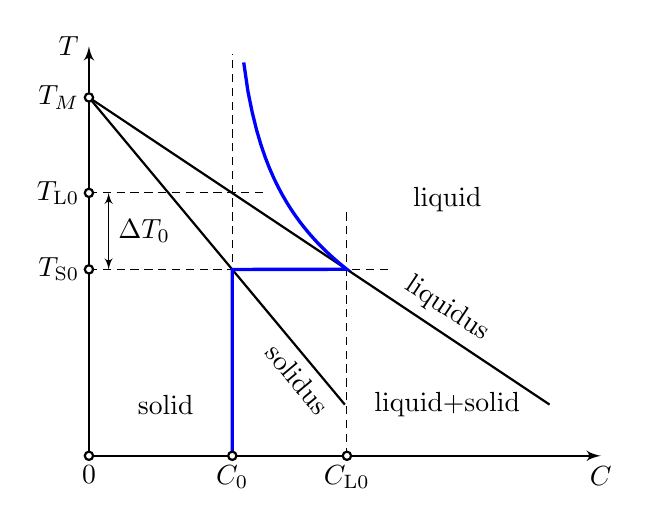
\begin{tikzpicture}[
            solution/.style={blue, very thick},
            boundary/.style={thick},
            mydashed/.style={densely dashed, shorten >=1mm},
            dot/.style = {thick, draw, fill=white, circle, inner sep=0pt, minimum size=3pt},
            >=latex', scale=1.3]

        \path (0,0) coordinate (origin) node[below] {0};
        \path (1.4,0) coordinate (C0) node[below] {$C_0$};
        \path (0,3.5) coordinate (TM) node[left] {$T_M$};

        \node at (0.75,0.5) {solid};
        \node at (3.5,0.5) {liquid+solid};
        \node at (3.5,2.5) {liquid};

        \draw[boundary,->] (origin) -- +(5,0) node[below] {$C$};
        \draw[boundary,->] (origin) -- +(0,4) node[left] {$T$};
        \draw[boundary,name path=liquidus] (TM) -- (4.5,0.5) node[near end, above, sloped] {liquidus};
        \draw[boundary,name path=solidus] (TM) -- (2.5,0.5) node[very near end, below, sloped] {solidus};
        \draw[mydashed,name path=lineC0] (C0) -- +(0,4);

        \path[name intersections={of=solidus and lineC0, by=intS}];
        \path (intS) -- (intS -| TM) coordinate (TS0) node[left] {$T_{\sol0}$};
        \draw[mydashed,name path=interface] (TS0) -- +(3,0);

        \path[name intersections={of=liquidus and lineC0, by=P}];
        \path (P) -- (P -| TM) coordinate (TL0) node[left] {$T_{\liq0}$};
        \draw[mydashed] (TL0) -- +(1.8,0);

        \path[name intersections={of=liquidus and interface, by=intL}];
        \path (intL) -- (intL |- C0) coordinate (CL0) node[below] {$C_{\liq0}$};
        \draw[mydashed] (CL0) -- +(0,2.5);

        \begin{scope}[transform canvas={xshift=0.25cm}]
            \draw[<->] (TL0) -- (TS0) node[midway,right] {$\Delta{T}_0$};
        \end{scope}

        \draw[solution] let \p1=($ (CL0)-(C0) $), \n1={veclen(\x1,\y1)*1pt/1cm}
            in (C0) -- (intS) -- (intL) -- plot[shift={(intL)}, domain=0:-\n1*0.9] (\x,{(ln(\n1)-ln(\x+\n1))*25});

        \node[dot] at (origin) {}; \node[dot] at (TM) {};
        \node[dot] at (C0) {}; \node[dot] at (CL0) {};
        \node[dot] at (TS0) {}; \node[dot] at (TL0) {};
    \end{tikzpicture}
    \caption{
        The phase diagram linearized for dilute binary alloys.
        The liquidus and solidus lines are given by equations $T=T_M + m_{\liq/\sol}C$.
        The blue line corresponds to the superimposed one-dimensional steady-state solution.
        Here, $C_0 = KC_{\liq0}$ is the initial solute concentration,
        $T_{\liq0}$ and $T_{\sol0}$ are the liquidus and solidus temperatures of the given alloy, respectively,
        $\Delta{T}_0 = (m_\liq-m_\sol)C_0$ is the solidification range.
    }
    \label{fig:binary:diagram}
\end{figure}

%%% Interface conditions
At the solid--liquid interface, the following conditions are satisfied up to $\order{\epsilon}$:
\begin{gather}
    \tilde{T}_\sol = \tilde{T}_\liq, \label{eq:BCT1}\\
    n\pdv{\tilde{T}_\sol}{z} - \pdv{\tilde{T}_\liq}{z}
        = \epsilon\zeta_x\qty(n\pdv{\tilde{T}_\sol}{x} - \pdv{\tilde{T}_\liq}{x}), \label{eq:BCT2}\\
    \tilde{C}_\sol = K\tilde{C}_\liq, \label{eq:BCC1}\\
    \pdv{\tilde{C}_\liq}{z} - \eta\pdv{\tilde{C}_\sol}{z}
        = \epsilon\zeta_x\qty(n\pdv{\tilde{T}_\liq}{x} - \pdv{\tilde{T}_\sol}{x})
        + (K-1)\tilde{C}_\liq(1+\epsilon\zeta_t), \label{eq:BCC2}\\
    \tilde{T}_\liq = 1 + M\tilde{C_\liq} + \gamma\epsilon\zeta_{xx}, \label{eq:BCgamma}
\end{gather}
where $M = m_\liq C_{\liq0}/T_M$ is the dimensionless liquidus slope,
which is assumed to have the same sign as the solidus one, i.e., $M(K-1) > 0$,
and $n = \kappa_\sol/\kappa_\liq$ is the thermal conductivity ratio.
Dimensionless capillary constant
\begin{equation}\label{eq:gamma}
    \gamma = \frac{\sigma V}{LD_\liq},
\end{equation}
where $\sigma$ is the surface tension (\si{\J\per\m\squared})
and $L$ is the latent heat of fusion (\si{\J\per\m\cubed}).

\subsection{Planar stationary solution}

\begin{figure}
    \centering
    \begin{gnuplot}[scale=0.8, terminal=epslatex, terminaloptions=color lw 5]
        set sample 1000
        set xrange [-1:1]
        set yrange [0.25:1.75]
        set key top center
        set grid
        K=0.5; M=0.1; G=0.5; n=1.5
        C(x) = x>0 ? 1 + (K-1)*(1-exp(-x)) : K
        T(x) = x>0 ? 1 + M + G*x : 1 + M + G*x/n
        plot C(x) title '$\tilde{C}$', T(x) title '$\tilde{T}$'
    \end{gnuplot}
    \caption{
        The one-dimensional steady-state solution of the solidification problem of a binary mixture
        for $K=0.5$, $M=0.1$, $\tilde{G}=0.5$, and $n=1.5$.
        The jump of the concentration at the interface given by Eq.~\eqref{eq:BCC1} is called \emph{solute rejection}.
    }
    \label{fig:binary:solution}
\end{figure}

By choosing the position of the front as the origin of the $z$ coordinate,
one finds the following planar stationary solution:
\begin{gather}
    \left.\begin{aligned}
        &\tilde{C}_\liq = 1 + (K-1)(1-e^{-z}), \\
        &\tilde{T}_\liq = 1 + M + \tilde{G}z,
    \end{aligned} \right\} \quad z > 0 \label{eq:solutionL}\\
    \left.\begin{aligned}
        &\tilde{C}_\sol = K, \hphantom{+(K-1)(1-e^{-z})}\\
        &\tilde{T}_\sol = 1 + M + \tilde{G}z/n,
    \end{aligned} \right\} \quad z < 0 \label{eq:solutionS}
\end{gather}
where $\tilde{G}T_MV/D_\liq$ is the temperature gradient in the liquid phase.
This solution is shown in Fig.~\ref{fig:binary:diagram} and~\ref{fig:binary:solution}.

\subsection{Linear stability analysis}

\begin{figure}
    \begin{adjustbox}{max width=1.2\linewidth,center}
        \begin{overpic}[width=0.6\textwidth]{binary/bifurcation}
            \put (5,90) {\adjustbox{minipage=0pt}{\subcaption{}\label{sfig:bifurcation}}}
        \end{overpic}
        \begin{overpic}[width=0.6\textwidth]{binary/bifurcation-log}
            \put (0,90) {\adjustbox{minipage=0pt}{\subcaption{}\label{sfig:bifurcation-log}}}
        \end{overpic}
    \end{adjustbox}
    \caption{
        The bifurcation diagram for the directional solidification of a binary mixture at $K=0.5$, $\eta=0$, and $n=1$.
        Both linear (\subref{sfig:bifurcation}) and logarithmic (\subref{sfig:bifurcation-log}) scales are shown.
        The maximum velocity given by~\eqref{eq:Vmax} is $\hV_\text{max} = 2$.
        The dashed line corresponds to the constitutional undercooling limit~\eqref{eq:Vmin},
        which takes the form $\hG = \hV_\text{min}$.
        The bifurcation curve has a single maximum $\hG_\text{max} = 0.09017$ at $\hV = 0.47214$ and $k = 0.63601$.
    }\label{fig:bifurcation}
\end{figure}

\begin{figure}
    \centering
    \includegraphics[width=0.8\textwidth]{binary/a0-G0.01-V0.1}
    \caption{
        The real part of the amplification factor $a_0(k)$ for a binary mixture at $\hG=0.01$ and $\hV=0.1$.
        There are two real solutions (blue and orange lines)
        and one complex solution (green line) of Eq.~\eqref{eq:binary:a0}.
        The smaller solution (orange line) can exist only in the gray area.
        Its lower boundary corresponds to a zero radicand in Eqs.~\eqref{eq:binary:qL} or~\eqref{eq:binary:qS},
        while the upper boundary marked by the dotted line is given by $\pdv*{\Delta}{a_0}=0$.
        Parameters $K$, $\eta$, and $n$ are specified in the caption of Fig.~\ref{fig:bifurcation}.
    }\label{fig:binary:a0}
\end{figure}

%%% Dispersion relation
By perturbing the planar solidification front harmonically as
\begin{equation}\label{eq:binary:perturbation}
    \epsilon\zeta(x,t) = \epsilon\exp(ikx + a_0t),
\end{equation}
one comes to the following dispersion relation:
\begin{equation}\label{eq:binary:a0}
    \Delta(a_0,k) = a_0 - \qL+1 + (\mathcal{G} + \beta k^2)(\qL-1 + K(\qS+1)) = 0,
\end{equation}
where
\begin{gather}
    \qL(a_0,k) = \frac12 + \qty(\frac14 + a_0 + k^2)^{\mathrlap{1/2}}, \label{eq:binary:qL}\\
    \qS(a_0,k) = -\frac12 + \qty(\frac14 + \eta a_0 + \eta^2k^2)^{\mathrlap{1/2}}, \label{eq:binary:qS}
\end{gather}
and
\begin{equation}\label{eq:Gbeta}
    \mathcal{G} = \frac{2\tilde{G}}{(n+1)M(K-1)}, \quad
    \beta = \frac{\gamma}{M(K-1)}.
\end{equation}

\begin{figure}
    \centering
    \vspace{-80pt}
    \includegraphics[width=\textwidth]{binary/lambdaGV}
    \caption{
        Stability of the wavelength $\hat\lambda=2\pi/\hV k$ as a function of $\hG$ and $\hV$.
        The gray surface corresponds to the neutral stability.
        The colored surface represents the most unstable wavelength with the amplitude $a_0$ displayed in the color bar.
        Parameters $K$, $\eta$, and $n$ are specified in the caption of Fig.~\ref{fig:bifurcation}.
    }\label{fig:binary:lambdaGV}
\end{figure}

%%% Change the dimensionless variables
In practice, for a given mixture, we can vary the temperature gradient and pulling speed in directional solidification.
Therefore, it is convenient to nondimensionalize them independently:
\begin{equation}\label{eq:hatGV}
    \hV = \frac{d_0}{\ell}, \quad \hG = \frac{d_0}{\ell_T},
\end{equation}
where
\begin{equation}\label{eq:lengths}
    d_0 = \frac{\Gamma}{\Delta{T}_0}, \quad
    \ell = \frac{D_\liq}{V}, \quad \ell_T = \frac{\Delta{T}_0}{G}
\end{equation}
are the chemical capillary, solute diffusion, and thermal lengths, respectively.
The quantity $\Gamma = \sigma T_M/L$ is called the Gibbs--Thomson coefficient,
and $\Delta{T}_0 = m_\liq C_0(K-1)/K$ is the freezing range of the alloy.
Substituting relations
\begin{equation}\label{eq:tildeGgamma}
    \tilde{G} = M(K-1)\hG/\hV, \quad \gamma = M(K-1)\hV
\end{equation}
into Eqs.~\eqref{eq:Gbeta}, we obtain
\begin{equation}\label{eq:Gbeta2}
    \mathcal{G} = 2\hG/(n+1)\hV, \quad \beta = \hV.
\end{equation}

%%% Bifurcation diagram
The typical bifurcation diagram in the ($\hV,\hG$) coordinates is shown in Fig.~\ref{fig:bifurcation}.
The planar front is stable for all wavenumbers when $\mathcal{G} > \mathcal{G}_c(\beta_c(k))$ given by
\begin{equation}\label{eq:bifurcation}
    \beta_c = \frac{K}{\mathcal{D}^2}\qty(\frac{\pS+1}{2\pL-1} - \eta^2\frac{\pL-1}{2\pS+1}), \quad
    \mathcal{G}_c = \frac{\pL-1}{\mathcal{D}} - \beta_c k^2,
\end{equation}
where $\pL(k)=\qL(0,k)$, $\pS(k)=\qS(0,k)$, and $\mathcal{D} = \pL-1 + K(\pS+1)$.
Eqs.~\eqref{eq:bifurcation} are obtained by taking $\Delta(0,k)=0$ and ${\pdv*{\Delta}{k^2}}(0,k)=0$.
In the \emph{absolute stability limit}~\cite{mullins1964stability} ($k\to0$),
\begin{equation}\label{eq:Vmax}
    \hV_\text{max} = 1/K.
\end{equation}
In the \emph{constitutional undercooling limit}~\cite{tiller1953redistribution} ($k\to\infty$),
$\lim_{k\to\infty}\beta_ck^2 = 0$, which gives
\begin{equation}\label{eq:Vmin}
    \hV_\text{min} = \frac{2(1+\eta K)}{n+1}\hG.
\end{equation}
Moving back to the dimensional variables, we have
\begin{equation}\label{eq:Vminmax}
    V_\text{min} = \frac{2(1+\eta K)}{n+1}\frac{GD_L}{\Delta{T}_0}, \quad
    V_\text{max} = \frac{D_L\Delta{T}_0}{K\Gamma}.
\end{equation}
The maximum point $\hG_\text{max}$ on the curve $\hG_c(\hV_c)$ can be found by adding
\begin{equation}\label{eq:Gmax}
    \mathcal{G}_c = \beta_c k^2
\end{equation}
to the system of equations~\eqref{eq:bifurcation}.
Eq.~\eqref{eq:Gmax} is obtained from
\begin{equation*}
    {\pdv{\Delta(a_0,k;\hV,\hG)}{\hV}}(0,k;\hV_c,\hG_c) = 0.
\end{equation*}

\begin{figure}
    \begin{adjustbox}{max width=1.4\linewidth,center}
        \begin{overpic}[width=0.7\textwidth]{binary/lambda-G0.01}
            \put (5,90) {\adjustbox{minipage=0pt}{\subcaption{}\label{sfig:binary:lambdaV1}}}
        \end{overpic}
        \begin{overpic}[width=0.7\textwidth]{binary/lambda-V0.1}
            \put (5,90) {\adjustbox{minipage=0pt}{\subcaption{}\label{sfig:binary:lambdaG1}}}
        \end{overpic}
    \end{adjustbox}
    \begin{adjustbox}{max width=1.4\linewidth,center}
        \begin{overpic}[width=0.7\textwidth]{binary/lambda-G0.0001}
            \put (5,90) {\adjustbox{minipage=0pt}{\subcaption{}\label{sfig:binary:lambdaV2}}}
        \end{overpic}
        \begin{overpic}[width=0.7\textwidth]{binary/lambda-V0.9}
            \put (5,90) {\adjustbox{minipage=0pt}{\subcaption{}\label{sfig:binary:lambdaG2}}}
        \end{overpic}
    \end{adjustbox}
    \caption{
        Stability of the wavelength $\hat\lambda=2\pi/\hV k$ as a function of $\hV$
        at $\hG=0.01$ (\subref{sfig:binary:lambdaV1}) and $\hG=0.0001$ (\subref{sfig:binary:lambdaV2})
        as well as a function of $\hG$
        at $\hV=0.1$ (\subref{sfig:binary:lambdaG1}) and $\hV=0.9$ (\subref{sfig:binary:lambdaG2}).
        Parameters $K$, $\eta$, and $n$ are specified in the caption of Fig.~\ref{fig:bifurcation}.
        The analytical and numerical models are given in Eqs.~\eqref{eq:cell_spacing} and~\eqref{eq:Hunt96}.
    }\label{fig:binary:lambda}
\end{figure}

%%% Amplification rate
For some point inside the unstable region in the bifurcation diagram (Fig.~\ref{fig:bifurcation}),
there is an interval of wavenumbers $(k_1,k_2)$
for which $a_0>0$ as shown in Fig.~\ref{fig:binary:a0}.
Note that for $\hG>0$, $k_1>0$ and, moreover, there is a critical wavenumber $k_c$
such that $a_0$ is complex for any $k<k_c$.

%%% Stability diagrams
We have seen that for $0<\hG<\hG_\text{max}$, there are two critical points, between which the planar front is unstable.
Stabilization is due to positive temperature gradient for longer wavelengths
and due to surface tension for shorter ones.
As a result, the neutral stability curve in the ($\hV,\hat\lambda$) coordinates
takes the oval shape as seen in Fig.~\ref{fig:binary:lambda}.

\subsection{Selection of the cell spacing}

%%% Cellular structures
The linear stability analysis enables us to predict conditions
under which a flat solidification front becomes unstable.
Moreover, we know the most unstable wavelength, which dominates during a linear perturbation.
However, the wavelength of a stable cellular structure cannot be found from this theory.

%%% Models for cell spacing
Two different models for the cell spacing are compared with the linear stability theory
in Fig.~\ref{fig:binary:lambda}.
The following models imply that $\eta=0$ and $n=1$.
First, a simple model can be formulated based on some ansatz for the shape of the solidification front.
For example, assuming that the solid is a dense hexagonal array of semi-ellipsoids,
we can obtain~\cite{rappaz2009solidification}
\begin{equation}\label{eq:cell_spacing}
    \hat\lambda^4 = \frac{72\pi^2}{K\hV\hG^2}.
\end{equation}
Second, \textcite{hunt1996numerical} employed a numerical model with dynamic spacing selection
and fitted their numerical results by
\begin{equation}\label{eq:Hunt96}
    \begin{gathered}
        \hat\lambda = 8.18 K^{-0.075}\hV^{-0.29}\qty(\hV - \hG)^{-0.3}\Delta\hat{T}_\sol^{-0.3}\qty(1-K\hV)^{-1.4}, \\
        \Delta\hat{T}_\sol = \hG/\hV + \qty(a + (1-a)\qty(K\hV)^{0.45})\qty(1-\hG/\hV), \\
        a = \num{5.273e-3} + 0.5519K - 0.1865K^2.
    \end{gathered}
\end{equation}

\subsection{Rapid solidification}

%%% Solute trapping and Aziz model
For high solidification rates, the planar solid--liquid interface is no longer in the equilibrium state.
The speed of solute diffusion becomes insufficient to equalize the chemical potential
with the corresponding concentration jump. In other words, solute atoms do not have enough time
to be rejected out of the solid and are therefore trapped in it.
This nonequlibrium phenomenon is called \emph{solute trapping}.
\textcite{aziz1982model} proposed a simple model for \emph{dilute} solutions to account for this effect
by introducing an effective partition coefficient
\begin{equation}\label{eq:Aziz}
    K_V = \frac{K + V/V_D}{1 + V/V_D},
\end{equation}
where $V_D$ is the so-called diffusion speed, which can be estimated as
\begin{equation}\label{eq:V_D}
    V_D = D_L/\delta_{\sol\liq},
\end{equation}
where $\delta_{\sol\liq}$ is the thickness of the diffuse interface.
In this sense, the dimensionless ratio $V/V_D$ can be interpreted as an interface P\'eclet number
and (cf.~Eq.~\eqref{eq:hatGV})
\begin{equation}\label{eq:hatV_D}
    \hV_D = d_0/\delta_{\sol\liq}.
\end{equation}
Eq.~\eqref{eq:Aziz} correctly describes both limits:
$K_V$ tends to the equilibrium value $K$ as $V/V_D\to0$ and to unity as $V/V_D\to\infty$.
The latter case corresponds to complete solute trapping, when diffusion can be ignored.

%%% Changing of slopes
It can be shown that the kinetic liquidus slope for a dilute solution
takes the form~\cite[see Appendix 6]{kurz1989fundamentals}
\begin{equation}\label{eq:mVL}
    m_{\liq V} = m_\liq\qty(1 + \frac{K - K_V(1+\ln(K/K_V))}{1-K}),
\end{equation}
which is consistent with Eq.~\eqref{eq:Aziz}.

\begin{figure}
    \begin{adjustbox}{max width=1.4\linewidth,center}
        \begin{overpic}[width=0.7\textwidth]{binary/lambda-rapid1}
            \put (5,90) {\adjustbox{minipage=0pt}{\subcaption{}\label{sfig:rapid1}}}
        \end{overpic}
        \begin{overpic}[width=0.7\textwidth]{binary/lambda-rapid0.1}
            \put (5,90) {\adjustbox{minipage=0pt}{\subcaption{}\label{sfig:rapid0.1}}}
        \end{overpic}
    \end{adjustbox}
    \caption{
        Stability of the wavelength $\hat\lambda=2\pi/\hV k$ as a function of $\hV$
        at $\hG=0.01$ for rapid solidification of a dilute binary mixture.
        Cases $\hV_D=1$ (\subref{sfig:rapid1}) and $\hV_D=0.1$ (\subref{sfig:rapid0.1}) are plotted.
        Case corresponding to the limit $\hV_D\to\infty$ is shown in Fig.~\ref{sfig:binary:lambdaV1}.
        Parameters $K$, $\eta$, and $n$ are specified in the caption of Fig.~\ref{fig:bifurcation}.
    }\label{fig:rapid}
\end{figure}

%%% Stability analysis
The linear stability analysis for a binary mixture remains valid in the case of rapid solidification.
The only amendment is that now the partition coefficient $K$ should be replaced by the kinetic one $K_V$,
which is a function of the velocity $\hV$.
For $K<1$, this correction leads to shrinking the area of instability as seen in Fig.~\ref{fig:rapid}.
This shrinkage is mainly observed in the region of larger $\hV$.
Given the dependence of $K_V(V)$, some of the above derived formulas should be also corrected.
In particular, the asymptotic relations~\eqref{eq:Vmax} and~\eqref{eq:Vmin} becomes nonlinear equations,
and Eq.~\eqref{eq:Gmax} is replaced by
\begin{equation}\label{eq:Gmax_rapid}
    \mathcal{G}_c = \beta_ck^2\frac{\mathcal{D} + K_V'\beta_c(p_\sol+1)}{\mathcal{D} - K_V'\beta_c(p_\sol+1)},
\end{equation}
where
\begin{equation}\label{eq:dK_V}
    K_V' = \frac{1-K}{\hV_D(1+V/V_D)^2}.
\end{equation}

\subsection{Extension to the multicomponent case}

%%% Assumptions
\textcite{coriell1987stability} have extended the presented theory to the multicomponent case
under the following assumptions:
\begin{enumerate}
    \item Solute diffusion in solid is absent ($\eta=0$).
    \item There is no diffusional interaction amongst solutes.
    \item The interface conditions are independent for each solute.
\end{enumerate}

%%% Dispersion relation
Let $m_{\liq i}$, $C_{0i}$, and $D_i$ be the liquidus slope, initial solute concentration,
and diffusion coefficient of the $i$th solute.
Its equilibrium solid--liquid concentration ratio is $K_i = m_{\liq i}/m_{\sol i}$.
Then the dispersion relation for an $(N+1)$-component mixture takes the form
\begin{equation}\label{eq:multi:a0}
    \Delta(a_0,k) = \sum_{i=1}^{N}I_i\frac{q_i - 1 - r_ia_0}{q_i - 1 + K_i} - g - k^2 = 0,
\end{equation}
where $r_i = D_i/D_0$, $D_0$ is the reference diffusion coefficient,
\begin{equation}\label{eq:multi:q}
    q_i(a_0,k) = \frac12 + \qty(\frac14 + r_ia_0 + (r_ik)^2)^{\mathrlap{1/2}},
\end{equation}
and
\begin{equation}\label{eq:multi:gI}
    g = \frac{\mathcal{G}}{\beta} = \frac{2D_0^2G}{(n+1)\Gamma V^2}, \quad
    I_i = \frac{D_0\Delta{T}_{0i}}{r_i\Gamma V}.
\end{equation}
Here, $\Delta{T}_{0i} = m_{\liq i}C_{0i}(K_i-1)/K_i$ is the $i$th contribution to the solidification range
$\Delta{T}_0 = \sum_i \Delta{T}_{0i}$.
Using the same definition of $\hV$ and $\hG$, given in~\eqref{eq:hatGV}, one can find that
\begin{equation}\label{eq:multi:gI2}
    g = \frac{2\hG}{(n+1)\hV^2}, \quad I_i = \frac{\Delta{T}_{0i}}{\Delta{T}_0}\frac1{r_i\hV}.
\end{equation}
It is easy to check that Eq.~\eqref{eq:multi:a0} reduces to Eq.~\eqref{eq:binary:a0} at $N=1$, $\eta=0$, $r_1=1$.

\printbibliography

\end{document}
